% natbib guide (https://gking.harvard.edu/files/natnotes2.pdf)
% \citet     #textual citations, print the abbreviated author list
% \citet*    #textual citations, print the full author list
% \citep     #parenthetical citations, print the abbreviated author list
% \citep*    #parenthetical citations, print the full author list
% \citealt    #the same as \citet but without any parentheses.
% \citealp    #the same as \citep but without any parentheses. 
% \citeauthor{ale91}         #Alex et al.
% \citeauthor*{ale91}        #Alex, Mathew, and Ravi
% \citeyear{ale91}           #1991 
% \citeyearpar{ale91}        #(1991)

\documentclass[spanish, xcolor=dvipsnames, aspectratio=169]{beamer}

% Text encoding
\usepackage[spanish]{babel}
\usepackage[draft]{pdfcomment}
\newcommand{\pdfnote}[1]{\marginnote{\pdfcomment[icon=note]{#1}}}
% Justify text (package and function)
% \apptocmd{command}{code}{success}{failure}
\usepackage{ragged2e}
\apptocmd{\frame}{}{\justifying}{} 
% Justify text in \item
\newcommand{\itemj}{\item \justifying}

% If...else package
\usepackage{ifthen}

% Package to set transparent background image
\usepackage{tikz}

% Include image package
\usepackage{graphicx}
% Set default path for images
\graphicspath{ {./imgs/} }
% Set figure number when included
\setbeamertemplate{caption}[numbered]

% Bibliography packages
\usepackage[sort, round]{natbib}
\bibliographystyle{plainnat}

% Define colors variables
\definecolor{red}{rgb}{0.631, 0.094, 0.094} % primary color
\definecolor{grey}{rgb}{0.3686, 0.5255, 0.6235} % secondary color

% Set theme palette colors
\setbeamercolor{palette primary}{bg=red,fg=white}
\setbeamercolor{palette secondary}{bg=red,fg=white}
\setbeamercolor{palette tertiary}{bg=red,fg=white}
\setbeamercolor{palette quaternary}{bg=red,fg=white}
% strucure means itemize, enumerate, etc
\setbeamercolor{structure}{fg=red} 

% Set bibliography colors
\setbeamercolor{bibliography item}{fg=red}
\setbeamercolor{bibliography entry author}{fg=black}
\setbeamercolor{bibliography entry title}{fg=black}
\setbeamercolor{bibliography entry location}{fg=black}
\setbeamercolor{bibliography entry note}{fg=black}
% Replaces book icon in bibliography with enumeration
\setbeamertemplate{bibliography item}{[\theenumiv]}

% Table of contents style
% \setbeamertemplate{section in toc}[sections numbered]
% \setbeamertemplate{subsection in toc}[subsections numbered]
\setbeamertemplate{section in toc}[circle]
\setbeamertemplate{subsection in toc}[ball unnumbered]

% Header with navigation bar
\setbeamertemplate{headline}
{
    \leavevmode
    \hbox{
    \begin{beamercolorbox}[wd=\paperwidth,ht=2.5ex,dp=1.125ex]{palette quaternary}
    \insertsectionnavigationhorizontal{\paperwidth}{}{\hskip0pt plus1filll}
    \end{beamercolorbox} 
    }
}
% Footer with custom caption
\setbeamertemplate{footline}
{
    \leavevmode
    \hbox{
    \begin{beamercolorbox}[wd=.33\paperwidth,ht=2.6ex,dp=1ex,center]{palette quaternary}
    \usebeamerfont{author in head/foot}\insertshortauthor\hspace*{1ex}
    \end{beamercolorbox}
    \begin{beamercolorbox}[wd=.33\paperwidth,ht=2.6ex,dp=1ex,center]{palette quaternary}
    \usebeamerfont{institute in head/foot}\insertshortinstitute
    \end{beamercolorbox}
    \begin{beamercolorbox}[wd=.33\paperwidth,ht=2.6ex,dp=1ex,center]{palette quaternary}
    \insertframenumber{} / \inserttotalframenumber
    \end{beamercolorbox}}
    \vskip0pt
}

% Global Background must be put in preamble
\usebackgroundtemplate
{
    \tikz\node[opacity=0.3]{
\includegraphics[height=\paperheight, width=\paperwidth]{white_background.jpg}};
}

% One line command to print table of contents - two parameters for modes
\newcommand{\customToC}[2]
{
    \begin{frame}{Contenido}
    \tableofcontents[#1, #2]
    \end{frame}
}

% Command to plot centered figure
% Parameters: #1=image name, #2=caption 
\newcommand{\includefigure}[2]
{
    \begin{figure}[h]
    \caption{#2}
    \centering
    \includegraphics[width=0.5\textwidth]{#1}
    \end{figure}
}

% Command to set section name as variable (\renewcommand to update)
\newcommand{\sectiontitle}{}
% Command to set subsection name as variable (\renewcommand to update)
\newcommand{\subsectiontitle}{}


% Title page
\title{Local Replacement and Scheduling: Ensemble Computation, Partition into Triangles, Sequencing with Intervals and Multiprocessor Scheduling}
\subtitle{Demostraciones de problemas NP-Completos}
\author{Rodrigo Arévalo Gaytán \and Fausto David Hernández Jasso}
\institute{Universidad Nacional Autónoma de México}
% Date
\day=01\relax
\month=10\relax
\year=2022\relax

\begin{document}

\frame{\titlepage}

% Complete table of contents (ToC)
% \customToC{hideallsubsections}{}
\customToC{hideothersubsections}{}

%%%%%%%%%%%%%%%%%%%%% PIT %%%%%%%%%%%%%%%%%%%%%%%%%%%
% Section name and highlighted ToC
\renewcommand{\sectiontitle}{Partition into Triangles}
\section{\sectiontitle}
\customToC{currentsection,hideothersubsections}{}

\begin{frame}{\sectiontitle}
    \begin{itemize}
        \itemj Ejemplar genérico: Una gráfica $G=(V,E)$, con $|V|=3q$ para un entero positivo $q$.
        \item Pregunta de decisión: Hay una partición de $V$ en $q$ conjuntos disjuntos $V_1,V_2,...,V_q$ de tres vértices cada uno tal que para cada $V_i=\{v_{i[1]},v_{i[2]},v_{i[3]}\}$, las tres aristas $\{v_{i[1]},v_{i[2]}\},\{v_{i[1]},v_{i[3]}\},\{v_{i[2]},v_{i[3]}\}$ pertenezcan a $E$?
    \end{itemize}
\end{frame}

\renewcommand{\subsectiontitle}{Algoritmo no determinista}
\subsection{\subsectiontitle}

\begin{frame}{\subsectiontitle}
    \begin{itemize}
    \itemj Fase Adivinadora\\
    \begin{itemize}
        \item Sabemos que $|V| = 3q$ entonces supongamos que tenemos un dado equilibrado de $q$ lados. Para cada $v\in V$ tiramos nuestro dado, sea $n$ el número obtenido por el dado, si el subconjunto de vértices $V_n$ tiene menos de 3 vértices entonces agregamos el vértice $v$ a $V_n$, si el subconjunto de vértices $V_n$ ya tiene 3 vértices entonces buscamos el siguiente $V_m$ que tenga menos de 3 vértices y agregamos $v$ a $V_m$, si llegamos a $V_q$ y no pudimos agregar a $v$ entonces desde $V_n$ buscamos el anterior $V_l$ que tenga menos de 3 vértices y agregamos $v$ a $V_l$, esto lo hacemos hasta recorrer por completo $V$.
    \end{itemize}
    

    \item Fase Verificadora\\

    \begin{itemize}
        \item Si la cardinalidad del conjunto de vértices de la gráfica $G$ no es múltiplo de 3 ningún candidato a solución será válido, entonces devolvemos NO en dicho caso.
        
        \item Si por cada subconjunto de 3 vértices $u,v,w \in V_i$ tenemos que las aristas\\ $(u,v),(u,w),(v,w)\in E$ entonces regresamos SI en otro caso regresamos NO.
    \end{itemize}

    
    
     
    
\end{itemize}
\end{frame}

% Section name and highlighted ToC
\renewcommand{\subsectiontitle}{Teorema y Demostración}
\subsection{\subsectiontitle}
% \customToC{currentsection,hideothersubsections}{}

\begin{frame}{\subsectiontitle}
    \begin{itemize}
        \itemj Teorema: El problema partición en traingulos es NP-Completo.
        \item Demostración: Transformamos cobertura exacta por conjuntos de 3 a partición en triangulos.
        \item Para demostrar el problema usaremos la técnica de reemplazo local. Pero primero ¿qué es la cobertura exacta por conjuntos de 3?
    \end{itemize}
\end{frame}

\renewcommand{\subsectiontitle}{Cobertura exacta por conjuntos de 3 (X3C)}
\subsection{\subsectiontitle}

\begin{frame}{\subsectiontitle}
    \begin{itemize}
        \itemj Ejemplar genérico: Un conjunto $X$ con $|X|=3q$ y una colección $C$ de subconjuntos de 3 elementos de $X$.
        \item Pregunta de decisión: ¿Existe algún subconjunto $C'$ de $C$ en donde cada elemento de $X$ aparezca \textbf{exactamente una vez} en $C'$? 
        \item Ejemplo: Supongamos que tenemos $X=\{1,2,3,4,5,6\}$.\\
        Si tenemos $C=\{\{1,2,3\},\{2,3,4\},\{1,2,5\},\{2,5,6\},\{1,5,6\}\}$, entonces podríamos elegir $C'=\{\{2,3,4\},\{1,5,6\}\}$ como cobertura exacta porque cada elemento de $X$ aparece \textbf{exactamente una vez}.
    \end{itemize}
\end{frame}

\renewcommand{\subsectiontitle}{Transformación}
\subsection{\subsectiontitle}

\begin{frame}{\subsectiontitle}
    \begin{itemize}
        \itemj Sea $X$ el conjunto con $|X|=3q$ y la colección $C$ de subconjuntos de 3 elementos de $X$ un ejemplar de $X3C$, construiremos una gráfica $G=(V,E)$ con
    $|V|=3q'$ tal que la partición deseada exista para $G$ si y solo si $C$ contiene una cobertura exacta.
        \item Las unidades básicas del ejemplar de $X3C$ son los subconjuntos de 3 elementos de $C$.
        \item El reemplazo local, por cada subconjunto $c_i=\{x_i,y_i,z_i\}\in C$, crea la siguiente gráfica:
    \end{itemize}
\end{frame}
\begin{frame}{\subsectiontitle}
    \begin{figure}
    \centering
        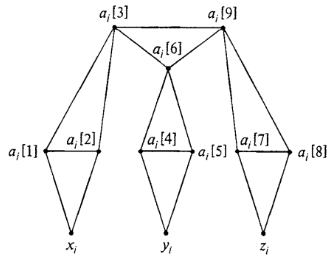
\includegraphics[width=.6\textwidth]{imgs/PIT/graficaPIT.png}
    \end{figure}
\end{frame}
\begin{frame}{\subsectiontitle}
    Así $G=(V,E)$ se define como
    \begin{align*}
        &V = X \cup \bigcup_{i=1}^{|C|} \{a_i[j]: 1\leqslant j\leqslant 9\}\\
        &E =\bigcup_{i=1}^{|C|}E_i
    \end{align*}

    Notemos que sólo los vértices que se conectan con aristas que pertenecen a más de un $E_i$ son aquellos que se encuentran en el conjunto $X$.\\

    \vspace{10pt}
    También podemos ver que $|V| = |X| + 9|C| = 3q + 9|C|$ así que $q'=q+3|C|$.
\end{frame}
\begin{frame}{Complejidad en tiempo de la transformación}
    La transformación del ejemplar de X3C al ejemplar de partición en triangulos se hace en tiempo polinomial. Tenemos que por cada subconjunto en $C$ se agregaran 12 vértices y 18 aristas a los respectivos conjuntos, lo que hace que la complejidad tenga $30|C|$ operaciones, lo que deja la complejidad en tiempo como $O(|C|)$.
\end{frame}

\begin{frame}{X3C = YES =$>$ PIT = YES}
    Si $c_1,c_2,...,c_q$, los subconjuntos de 3 elementos de $C$, están en alguna cobertura exacta para $X$, entonces la partición correspondiente $V=V_1 \cup V_2 \cup ... \cup V_q$ de $V$ está dada al tomar
    \begin{align*}
        \{a_i[1],a_i[2],x_i\},\{a_i[4],a_i[5],y_i\},\{a_i[7],a_i[8],z_i\}, \{a_i[3],a_i[6],a_i[9]\}
    \end{align*}
    de los vértices conectados por $E_i$ cuando $c_i=\{x_i,y_i,z_i\}$ está en la cobertura exacta.\\

    \vspace{10pt}
    Y tomando
    \begin{align*}
        \{a_i[1],a_i[2],a_i[3]\},\{a_i[4],a_i[5],a_i[6]\},\{a_i[7],a_i[8],a_i[9]\}
    \end{align*}
    de los vértices conectados por $E_i$ cuando $c_i=\{x_i,y_i,z_i\}$ no está en la cobertura exacta. Esto asegura que cada elemento de $X$ este incluido en exactamente un subconjunto de 3 vértices en la partición\\
\end{frame}

\begin{frame}{X3C = YES $<$= PIT = YES}
    Si $V_1\cup V_2 \cup ... \cup V_q$ es una partición en triangulos de $G$, la cobertura exacta está dada al elegir los $c_i\in C$ tal que $\{a_i[3],a_i[6],a_i[9]\}=V_j$ para alguna j, $1\leqslant j \leqslant q'$
\end{frame}

\renewcommand{\subsectiontitle}{Ejemplo de transformación}
\subsection{\subsectiontitle}

\begin{frame}{\subsectiontitle}
    Supongamos que tenemos un ejemplar de X3C con un conjunto $X=\{1,2,3,4,5,6\}$ y una colección $C=\{\{1,4,6\},\{2,4,6\},\{2,3,5\}\}$, entonces nuestro ejemplar de partición en triángulos nos quedaría como
\end{frame}
\begin{frame}
    \begin{figure}
    \centering
        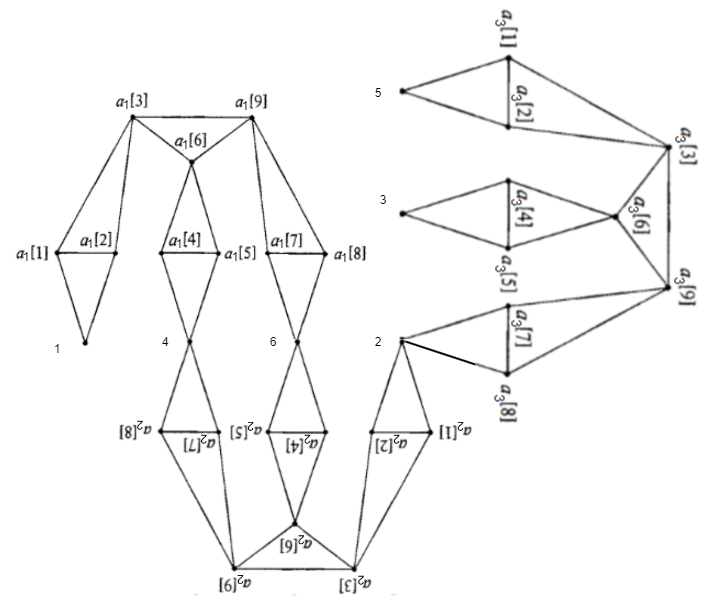
\includegraphics[width=.7\textwidth]{imgs/PIT/EjemploPIT.png}
    \end{figure}
\end{frame}

% Section name and highlighted ToC
\renewcommand{\sectiontitle}{Ensemble Computation}
\section{\sectiontitle}
\customToC{currentsection,hideothersubsections}{}

% Section name and highlighted ToC
\renewcommand{\subsectiontitle}{Forma canónica o estándar}
\subsection{\subsectiontitle}
\begin{frame}{\subsectiontitle}
    \begin{itemize}
        \item \textbf{Ejemplar genérico: } Una colección $C$ de subconjuntos de un conjunto 
              finito $A$ y un entero positivo $J$.
        \item \textbf{Pregunta de decisión: } ¿Existe una secuencia
        \[
            \langle z_{1} = x_{1} \cup y_{1}, z_{2} = x_{2} \cup y_{2}, \dotsc, z_{j} =  x_{j} \cup y_{j} \rangle
        \]
        con $j$ operaciones de unión, tal que $j \leq J$, donde cada $x_{i}$ y $y_{i}$ es $\{ a \}$ para algún $a \in A$ o es $z_{k}$ para alguna $k < i$, además $x_{i}$ y $y_{i}$ son 
        disjuntos para todo $1 \leq i \leq j$, para todo subconjunto $c \in C$ existe alguna 
        $z_{i}$ con $1 \leq i \leq j$, tal que $z_{i}$ es igual a $c$?
    \end{itemize}
\end{frame}
\renewcommand{\subsectiontitle}{Entendiendo el enunciado}
\subsection{\subsectiontitle}
\begin{frame}{\subsectiontitle}
\begin{itemize}
    \item $A$ es un conjunto finito.
    \item $C$ es una colección formado por subconjuntos de $A$, es decir, para todo \(c\) en la colección 
          \(c \in \mathcal{P}\left(A\right)\)
    \item Cada $x_{i}$ y $y_{i}$ son conjuntos, como los describimos anteriormente sí $x_{i}$ y $y_{i}$ no es de la forma $\{ a \}$ para algún $a \in A$, entonces son un elemento $z_{k}$ \textit{``anterior``} de la secuencia.
    \item Se busca que la secuencia cumpla que para todo elemento $c \in C$ siempre debe de existir un elemento de la secuencia que sea idéntico a él, es decir, sí $c \in C$ entonces existe $z_{k}$ tal que:
    \begin{itemize}
        \item $z_{k}$ forma parte de la secuencia.
        \item $z_{k} = c$.
    \end{itemize}
\end{itemize}
\end{frame}
\renewcommand{\subsectiontitle}{Ejemplo}
\subsection{\subsectiontitle}
\begin{frame}{\subsectiontitle}
\begin{itemize}
    \item Sea \(A = \{a, b, c, d, e\}\), \(C = \{\{a, b\}, \{b, c, d\}, \{c, e\}\}\) y \(J = 4\).
    \item Una secuencia que cumple lo que nos pide el problema es:
            \[
                \langle z_{1} = \{a, b\}, z_{2} = \{b, c\}, z_{3} = \{b, c, d\}, z_{4} = \{c, e \} \rangle
            \]
    \item En la secuencia anterior, notemos que se cumple \(j \leq J\).
    \item En la secuencia anterior \(x_{i}\) y \(y_{i}\) para \(1 \leq i \leq j\) con \(j = 4\) están dados por:
    \begin{itemize}
        \item \(x_{1} = \{a\}\), \(y_{1} = \{b\}\) ya que \(z_{1} = x_{1} \cup y_{1} = \{a\} \cup \{b\} = \{a, b\}\)
        \item \(x_{2} = \{b\}\), \(y_{2} = \{c\}\) ya que \(z_{2} = x_{2} \cup y_{2} = \{b\} \cup \{c\} = \{b, c\}\)
        \item \(x_{3} = z_{2}\), \(y_{3} = \{d\}\) ya que \(z_{3} = x_{3} \cup y_{3} = z_{2} \cup y_{3} = \{b, c\} \cup \{d\} = \{b, c, d\}\).
        \item \(x_{4} = \{c\}\), \(y_{4} = \{e\}\) ya que \(z_{4} = x_{4} \cup y_{4} = \{c\} \cup \{e\} = \{c, e\}\)
    \end{itemize}
    Consecuentemente se cumple que para todo \(x_{i}\) y \(y_{i}\) para \(1 \leq i \leq 4\) es de la forma $\{ a \}$ para algún $a \in A$ o 
    es $z_{k}$ para alguna $k < i$.
    \end{itemize}
\end{frame}
\begin{frame}{\subsectiontitle}
    Notemos que \(x_{i} \cap y_{i} = \varnothing\) ya que:
    \begin{itemize}
        \item \(x_{1} \cap y_{1} = \{a\} \cap \{b\} = \varnothing\)
        \item \(x_{2} \cap y_{2} = \{b\} \cap \{c\} = \varnothing\)
        \item \(x_{3} \cap y_{3} = z_{2} \cap y_{3} = \{b, c\} \cap \{d\} = \varnothing\).
        \item \(x_{4} \cap y_{4} = \{c\} \cap \{e\} = \varnothing\)
    \end{itemize}
    Por lo tanto se cumple que para todo \(x_{i}\) y \(y_{i}\) son disjuntos.
\end{frame}
\begin{frame}{\subsectiontitle}
    Nombraremos a los elementos del conjunto \(C\)
    \begin{align*}
        c_{1} &= \{a, b\} \\
        c_{2} &= \{b, c, d\} \\
        c_{3} &= \{c, e\}
    \end{align*}
    Así notemos que 
    \begin{align*}
        c_{1} &= z_{1} \\
        c_{2} &= z_{3} \\
        c_{3} &= z_{4}
    \end{align*}
    Por lo tanto se cumple que para todo \(c \in C\) existe \(z_{k}\) en la secuencia tal que \(c = z_{k}\), así la secuencia cumple con 
    lo solicitado por el problema.
\end{frame}
\renewcommand{\subsectiontitle}{Algoritmo no determinista}
\subsection{\subsectiontitle}
\begin{frame}{\subsectiontitle}
    \begin{itemize}
        \item Fase adivinadora:
        \begin{itemize}
            \item Sea $S$ una secuencia vacía
            \item Pondremos todos los elementos de la colección \( C \) en un frasco.
            \item Tenemos un dado equilibrado con $|C|$ caras.
            \item Tiramos el dado y obtendremos un número \( j \) tal que \( j \in \{1, 2, \dotsc, |C| \}\).
            \item Sacaremos $j$ conjuntos de la colección $C$ de la siguiente manera:
            \begin{itemize}
                \item Al sacar el \(i\)-ésimo conjunto $c$ del frasco lo agregamos a la secuencia $S$ y nos referiremos a éste como $z_{i}$.
                \item Para $x_{i}$ tomamos un subconjunto de $c$ tal que sea de cardinalidad $1$.
                \item Para $y_{i}$ tomamos el subconjunto restante de $c$.
            \end{itemize}
        \end{itemize} 
        \item Fase verificadora:
        \begin{itemize}
            \item Si $|C| > J$ entonces no habrá solución para el ejemplar, en otro caso verificamos que la secuencia cumpla las restricciones, si $S$ no cumple alguna, entonces $S$ no es una solución para el ejemplar, si $S$ cumple todas las restricciones entonces sí una solución para el ejemplar.
        \end{itemize}
    \end{itemize}
\end{frame}
\renewcommand{\subsectiontitle}{Complejidad del algoritmo no determinista}
\subsection{\subsectiontitle}
\begin{frame}{\subsectiontitle}
    \begin{itemize}
        \item Fase adivinadora:
        \begin{itemize}
            \item Agregar elementos a la secuencia nos toma $O\left(|C|\right)$ ya que en el peor de los casos $j = |C|$.
            \item Definir a cada $x_{i}$ y $y_{i}$ con $1 \leq i \leq j$ nos toma $O\left(|C|\right)$.
        \end{itemize}
        \item Fase verificadora:
        \begin{itemize}
            \item Comprobar que $j \leq J$ nos toma $O\left(1\right)$.
            \item Comprobar que cada $x_{i}$ y $y_{i}$ cumple con la forma solicitada nos toma tiempo $O\left(|C| + |A|\right)$ ya que existen $j$ de cada uno de ellos entonces debemos comprobar $2j$ conjuntos que cumplan con lo solicitado, recordemos que éstos su vez pueden tener dos formas:
            \begin{itemize}
                \item $\{ a \}$ con $a \in A$.
                \item $z_{k}$ con $k < i$.
            \end{itemize}
            así la complejidad de éste paso es $O\left(|C| \cdot \left(|C| + |A|\right)\right)$.
            \item Comprobar que para cada $c \in C$ existe un elemento de la secuencia $z_{i}$
            tal que $z_{i} = c$ está dado por $O\left( j \cdot |C| \right)$.
            \item Comprobar que cada $x_{i} \cap y_{i} = \varnothing$ nos toma $j$ operaciones
            ya que hay $j$ $x_{i}$ y $j$ $y_{i}$ por lo tanto nos toma ésta comprobación tiempo $O\left(|C|\right)$.
        \end{itemize}
    \end{itemize}
\end{frame}
\renewcommand{\subsectiontitle}{Vertex cover (Cobertura de vértices)}
\subsection{\subsectiontitle}
\begin{frame}{\subsectiontitle}
Definición:
\newline
Una cobertura de vértices es un subconjunto \(V'\) de vértices de la gráfica \(G = \left(V, E\right) \) tal que para cada 
arista \( \left(u, v\right) \in E \), \(u \in V'\) ó \(v \in V'\).
\end{frame}
\begin{frame}{Ejemplo}
    \begin{figure}
        \centering
        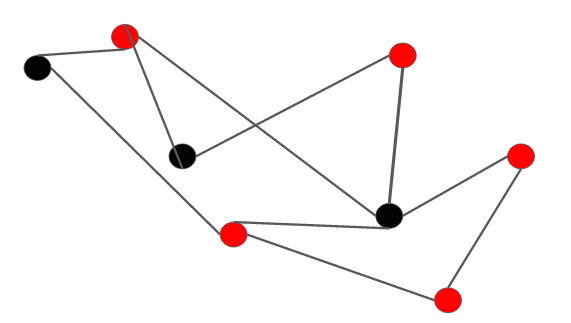
\includegraphics[scale = 0.5]{imgs/EC/Vertex Cover/Examples/mWdKEnYasQ-screen-shot-2016-07-05-at-85407-pm.png}
        \caption{Gráfica \( G \)}
    \end{figure}
\end{frame}
\begin{frame}{Ejemplo}
    En la gráfica \( G \), el conjunto de vértices de color rojo, forma una cobertura de vértices en \( G \) mientras que el conjunto de vértices de 
    color negro no.
\end{frame}
\begin{frame}{Problema de la cobertura de vértices}
    Dada una gráfica \(G\) y un entero positivo \(M\), ¿\(G\) tiene una cobertura de vértices de tamaño a lo más \(M\)?
    \newline 
    El problema de la \textbf{cobertura de vértices} es \textbf{NP-}Completo
\end{frame}

\renewcommand{\subsectiontitle}{Teorema}
\subsection{\subsectiontitle}
\begin{frame}{\subsectiontitle}
El problema \textbf{Ensemble Computation} es \textbf{NP}-Completo
\end{frame}
\renewcommand{\subsectiontitle}{Demostración}
\subsection{\subsectiontitle}
\begin{frame}{\subsectiontitle}
Transformaremos \textbf{Vertex Cover} a \textbf{Ensemble Computation}.
\newline 
Sea \(G = \left(V, E\right)\) una gráfica tal que:
\begin{itemize}
    \item \(V\) es el conjunto de vértices de la gráfica.
    \item \(E\) es el conjunto de aristas de la gráfica.
\end{itemize}
y sea \(K\) un entero positivo tal que \(K \leq |V|\), lo anterior es un ejemplar genérico de \textbf{Vertex Cover}.
\end{frame}
\begin{frame}{\subsectiontitle}
    Sea \(a_{0}\) un elemento nuevo tal que \(a_{0} \notin V\). Entonces para cada arista \(\{u, v\} \in E\) formamos el conjunto 
    \(\{a_{0}, u, v\}\), el conjunto que contiene a todos éstos conjuntos descritos anteriormente, lo nombraremos como conjunto \(C\).
    Es decir, \(C\) está definido de la siguiente manera:
    \[
        C = \{ \{a_{0}, u, v\} \ | \ \{u, v\} \in E\} 
    \]
    Definimos al conjunto \(A\) como \(A = V \cup \{a_0\}\)
    \newline
    Definimos al entero \(J\) como \(J = K + |E|\), notemos que \(J \in \mathbb{Z}^{+}\) ya que \(K \in \mathbb{Z}^{+}\) y \(|E| \in \mathbb{Z}^{+}\)
\end{frame}
\begin{frame}{\subsectiontitle}
    Ahora lo que tenemos es un ejemplar genérico de \textbf{Ensemble Computation}. Éste ejemplar se construyó en tiempo polinomial ya que:
    \begin{itemize}
        \item Formar el conjunto \(A\) nos tomó \(|V| + 1\) operaciones así la complejidad en tiempo de la construcción está dada por \(O\left(|V|\right)\).
        \item Formar el conjunto \(C\) nos tómo \(|E|\) operaciones así la complejidad en tiempo en la construcción está dada por \(O\left(|E|\right)\), a su vez
        \(|E|\) está acotado por  \(O\left(|V|^2\right)\) ya que el mayor número de aristas que puede tener una gráfica está dado por \(\frac{|V|\left(|V| - 1\right)}{2}\)
        \textit{(Gráfica completa)}.
        \item Formar el número \(J\) se hace en tiempo constante \(O\left(1\right)\) ya que siempre se efectúan dos operaciones.
    \end{itemize}
\end{frame}
\begin{frame}{\subsectiontitle}
    \textbf{Afirmación:}
    \newline
    \textit{\(G\) tiene una cobertura de vértices de a los más \(K\) sí y sólamente sí existe la secuencia deseada de \(j \leq J\) operaciones 
    para el conjunto \(C\)}
\end{frame}
\begin{frame}{\subsectiontitle}
    \textbf{Ida}
    \newline
    Supongamos que \(V'\) es una cobertura de vértices para la gráfica \(G\) y \(|V'| \leq K\). Notemos que podemos agregar vértices a \(V'\) y continuará 
    siendo una cobertura de vértices. Sin pérdida de generalidad asumiremos que \(|V'| = K\). Nombramos los elementos de \(V'\) como 
    \(v_{1}, v_{2}, \dotsc, v_{K}\) y etiquetamos a las aristas en \(E\) como \(e_{1}, e_{2}, \dotsc, e_{m}\) donde \(m = |E|\). 
\end{frame}
\begin{frame}{\subsectiontitle}
    Ya que \(V'\) es una cobertura de vértices 
    entonces cada arista \(e_{j}\) contiene al menos un elemento de \(V'\). Consecuentemente podemos escribir a \(e_{j}\) como 
    \[
        e_{j} = \{u_{j}, v_{r\left[j\right]}\}
    \]
    donde \(r\left[j\right]\) es un entero tal que \(1 \leq r\left[j\right] \leq K\). La siguiente secuencia:
    \begin{align*}
        \langle z_{1} &=\{a_{0}\} \cup \{v_{1}\}, z_{2} = \{a_{0}\} \cup \{v_{2}\}, \dotsc, z_{K} = \{a_{0}\} \cup \{v_{K}\}, \\
                        z_{K + 1} &= \{u_{1}\} \cup z_{r\left[1\right]}, z_{K + 2} = \{u_{2}\} \cup z_{r\left[2\right]}, \dotsc, z_{J} = \{u_{m}\} \cup z_{r\left[m\right]} \rangle  
    \end{align*}
    cumple con los propiedades solicitadas por \textbf{Ensemble Computation}.
\end{frame}
\begin{frame}{\subsectiontitle}
    \textbf{Regreso}
    \newline
    Supongamos que \(S\) es la secuencia deseada es decir, definimos a \(S\) como 
    \[
        S = \langle z_{1} = x_{1} \cup y_{1}, \dotsc, z_{j} = x_{j} \cup y_{j}  \rangle  
    \]
    con \(j \leq J\). Supondremos que \(S\) es la secuencia que contiene el menor número de operaciones de la forma \(z_{i} = \{ u \} \cup \{ v \}\)
    para \(u, v \in V\). Notemos que \(S\) no puede contener operaciones de ésta forma.
\end{frame}
\begin{frame}{\subsectiontitle}
    Supongamos que \(z_{i} = \{ u \} \cup \{ v \}\) con 
    \(u, v \in V\).
    \newline 
    Notemos que \(\{u, v\} \notin C\) ya que por construcción los elementos de \(C\) son de la forma \(\{a_0, u, v\}\) con \(a_0\) un 
    nuevo elemento, y \(\{u, v\} \in E\), de nuevo por construcción debe ocurrir que \(\{u, v\} \in E\). 
    \newline
    Como \(S\) cumple con las condiciones dadas 
    entonces debe de existir una \(z_{j} = \{a_{0}, u, v\}\) ya que \(\{a_0, u, v\} \in C\), como \(z_{i} = \{u, v\}\) entonces \(z_{j} = \{a_{0}\} \cup z_{i}\)
    y por ende \(i < j\), es decir \(z_{j}\) aparece ``después`` en \(S\). 
    \newline
    Por construcción tenemos \(\{u, v\}\) es subconjunto de un solo elemento de \(C\).
    Así \(z_i\) no puede ser usado en ningún elemento de la secuencia más que en \(z_{j}\).
\end{frame}
\begin{frame}{\subsectiontitle}
    Notemos lo siguiente
    \begin{align*}
        z_{i} &= \{u\} \cup \{v\} &\text{y}& & z_{j} = \{a_0, u, v\} = \{a_0\} \cup z_{i}
    \end{align*}
    Podemos redefinirlo como:
    \begin{align*}
        z_{i} &= \{a_0\} \cup \{u\} &\text{y}&  & z_{j} = \{a_0, u, v\} = \{v\} \cup z_{i}
    \end{align*}
\end{frame}
\begin{frame}{\subsectiontitle}
    Observemos que seguimos cumpliendo las restricciones impuestas por el problema, lo anterior implica que 
    hemos encontrado una secuencia \(S'\) con menor número de operaciones de tipo \(\{u\} \cup \{v\}\) lo cual es una contradicción.
    Por lo tanto las operaciones en \(S\) solamente tienen dos formas:
    \begin{itemize}
        \item \(z_{i} = \{a_0\} \cup \{u\}\) para \(u \in V\)
        \item \(\{a_0, u, v\} = \{v\} \cup z_{i}\) para \(\{u, v\} \in E\)
    \end{itemize}
\end{frame}
\begin{frame}{\subsectiontitle}
    De nuevo, por construcción tenemos \(|C| = |E|\), como todo \(c \in C\) debe de ser igual a un \(z_{k}\) de \(S\) entonces 
    \(S\) contiene exactamente \(|E|\) operaciones del tipo \(\{a_0, u, v\}\). Observamos que
    \begin{align*}
        j &\leq J \\
        j - |E| &\leq J - |E| \\
    \end{align*}
    Definimos a \(K\) como \(J - |E|\), y tenemos a lo más \(K\) de operaciones de la forma \(\{a_0\} \cup \{u\}\).
    \newline 
    Ahora definiremos al conjunto \(V'\) que describe las operaciones anteriores, es decir 
    \[
        V' = \{\{a_0\} \cup \{u\} \ | \ u \in V \}  
    \]
    Consecuentemente \(|V'| \leq K\) como cada \(\{a_0, u\}\) es un subconjunto de algún elemento de \(C\), entonces 
    \(V'\) es una cobertura de vértices de \(G\).
\end{frame}
\renewcommand{\subsectiontitle}{Ejemplificación de la transformación}
\subsection{\subsectiontitle}
\begin{frame}{\subsectiontitle}
Consideremos la gráfica \(G = \left(V, E\right)\) definida como sigue:
\begin{align*}
    V = &\{v_{1}, v_{2}, v_{3}, v_{4}, v_{5}, v_{6}, v_{7}, v_{8}\} \\
    E = &\{\{v_{1}, v_{2}\}, \{v_{1}, v_{5}\}, \{v_{2}, v_{5}\}, \{v_{2}, v_{6}\}, \{v_{2}, v_{3}\}, \\
        &\{v_{2}, v_{7}\}, \{v_{3}, v_{4}\}, \{v_{4}, v_{7}\}, \{v_{4}, v_{8}\}, \{v_{5}, v_{6}\}\}
\end{align*}
Observamos que:
\begin{align*}
    |V| &= 8 \\
    |E| &= 10
\end{align*}
Una cobertura de vértices para \(G\) es el conjunto \(V'\) definido como sigue:
    \[
        V' = \{v_{2}, v_{4}, v_{5}\}  
    \]
Nuestro entero positivo es \(K = 3\).
\end{frame}
\begin{frame}{\subsectiontitle}
    Sea \(a_0\) un nuevo elemento, claramente se cumple que \(a_{0} \notin V\). Formamos el conjunto \(C\) de la siguiente forma:
    \begin{align*}
        C = \{ &\{a_{0}, v_{1}, v_{2}\}, \{a_{0}, v_{1}, v_{5}\}, \\
               &\{a_{0}, v_{2}, v_{5}\}, \{a_{0}, v_{2}, v_{6}\}, \\
               &\{a_{0}, v_{2}, v_{3}\}, \{a_{0}, v_{2}, v_{7}\}, \\
               &\{a_{0}, v_{3}, v_{4}\}, \{a_{0}, v_{4}, v_{7}\}, \\
               &\{a_{0}, v_{4}, v_{8}\}, \{a_{0}, v_{5}, v_{6}\}\}
    \end{align*}
    Definimos a \(A\) como
    \[
        A = V \cup \{a_{0}\} = \{v_{1}, v_{2}, v_{3}, v_{4}, v_{5}, v_{6}, v_{7}, v_{8}, a_0\}
    \]
    Notemos que todo \(c \in C\) cumple con \(c \in \mathcal{P}\left(A\right)\)
    \newline 
    Definimos a \(J\) como
    \[
        J = K + |E| = 3 + 10 = 13
    \]
    Así tenemos un ejemplar genérico de \textbf{Ensemble Computation.}
\end{frame}
\renewcommand{\subsectiontitle}{Técnica para la demostración del problema}
\subsection{\subsectiontitle}
\begin{frame}{\subsectiontitle}
Reemplazo Local
\end{frame}
\renewcommand{\subsectiontitle}{Aplicación en la vida real}
\subsection{\subsectiontitle}
\begin{frame}{\subsectiontitle}
\begin{itemize}
    \item Encontrar circuitos con el menor número de compuertas lógicas.
    \item Encontrar una manera eficiente de realizar determinadas multiplicaciones entre números, matrices, etc.
\end{itemize}
\end{frame}
% \renewcommand{\subsectiontitle}{Teorema}
% \subsection{\subsectiontitle}
% \begin{frame}{\subsectiontitle}
% El problema \textbf{Ensemble Computation} es \textbf{NP}-Completo
% \end{frame}

%%%%%%%%%%%%%%%%%% PARTE RAG %%%%%%%%%%%%%%%%%%%%%%%%

%%%%%%%%%%%%%%%%%%%%% SWI %%%%%%%%%%%%%%%%%%%%%%%%%%%
\renewcommand{\sectiontitle}{Sequencing within intervals}
\section{\sectiontitle}
\customToC{currentsection,hideothersubsections}{}

\begin{frame}{\sectiontitle}
    \begin{itemize}
        \itemj Ejemplar genérico: Un conjunto finito $T$ de tareas y por cada $t\in T$, un entero \textit{tiempo de liberación} $r(t)\geqslant 0$, un \textit{tiempo limite} $d(t)\in \mathrm{Z}^+$ y una longitud $l(t)\in \mathrm{Z}^+$.
        
        \item Pregunta de decisión: ¿Existe un horario factible para $T$, una función $\sigma:T\to \mathrm{Z}^+$ tal que para cada $t\in T$, $\sigma(t)\geqslant r(t), \sigma(t) + l(t)\leqslant d(t)$ y si $t'\in T-\{t\}$ entonces $\sigma(t')+l(t') \leqslant \sigma(t)$ o $\sigma(t') \geqslant \sigma(t) + l(t)$ ?\\
        (la tarea $t$ es ejecutada desde el tiempo $\sigma(t)$ al tiempo $\sigma(t) + l(t)$, no se puede ejecutar hasta el tiempo $r(t)$, debe ser completada para el tiempo $d(t)$ y su ejecución no puede traslaparse con la ejecución de otra tarea $t'$).
    \end{itemize}
\end{frame}

\renewcommand{\subsectiontitle}{Algoritmo no determinista}
\subsection{\subsectiontitle}

\begin{frame}{\subsectiontitle}
    \begin{itemize}
    \itemj Fase Adivinadora\\
    \begin{itemize}
        \item Tiramos un dado equilibrado de $|T|$ lados y del número $n$ que salga tomamos la tarea $t_n$ del conjunto $T$, la renombramos como $t_1'$ hacemos su horario factible igual a $\sigma(t_1')=0$ volvemos a tirar el dado y del número $m$ que salga tomamos la tarea $t_m$ del conjunto $T$, y la renombramos como $t_2'$, hacemos el $\sigma (t_2') = \sigma(t_1') + l(t_1')$, ..., volvemos a tirar el dado y del número $j$ que salga tomamos la tarea $t_j$ del conjunto $T$, y la renombramos como $t_i'$, tal que $t_{i-1}'$ sea la tarea anterior a la que le asignamos su horario factible, hacemos el $\sigma (t_i') = \sigma(t_{i-1}') + l(t_{i-1}')$, y hacemos esto hasta asignarle un horario factible a la tarea $t_{|T|}$.
    \end{itemize}
    
    \item Fase Verificadora\\
    \begin{itemize}
        \item Por cada tarea verificamos que $\sigma(t)\geqslant r(t), \sigma(t) + l(t)\leqslant d(t)$ y si $t'\in T-\{t\}$ entonces $\sigma(t')+l(t') \leqslant \sigma(t)$ o $\sigma(t') \geqslant \sigma(t) + l(t)$, si se cumple para todas las tareas devolvemos SI, en otro caso regresamos NO.
    \end{itemize}
    
    
\end{itemize}
\end{frame}

\renewcommand{\subsectiontitle}{Teorema y Demostración}
\subsection{\subsectiontitle}
% \customToC{currentsection,hideothersubsections}{}

\begin{frame}{\subsectiontitle}
    \begin{itemize}
        \itemj Teorema: El problema secuenciación dentro de intervalos es NP-Completo.
        \item Demostración: Transformamos partición a secuenciación dentro de intervalos.
        \item Para demostrar el problema usaremos la técnica de reemplazo local. Pero primero ¿qué es el problema de partición?
    \end{itemize}
\end{frame}

\renewcommand{\subsectiontitle}{Partición}
\subsection{\subsectiontitle}

\begin{frame}{\subsectiontitle}
    \begin{itemize}
        \itemj Ejemplar genérico: Un multiconjunto $S$ de enteros positivos.
        \item Pregunta de decisión: Existen 2 subconjuntos $S_1$ y $S_2$ tal que la suma de los enteros de $S_1$ sea igual a la suma de los enteros de $S_2$?
        \item Ejemplo:
        Supongamos que tenemos $S=\{3,1,1,2,2,1\}$.\\
        Sea $S_1=\{1,1,1,2\}$ y $S_2=\{2,3\}$ vemos que ambos subconjuntos suman 5 y devuelven YES a la pregunta de decisión. Podemos ver que otra partición la tenemos con los subconjuntos $S_1=\{3,1,1\}$ y $S_2=\{2,2,1\}$ vemos que ambos subconjuntos suman 5.
        \item Dato curioso: Este problema es llamado el problema difícil más fácil.
    \end{itemize}
\end{frame}

\renewcommand{\subsectiontitle}{Transformación}
\subsection{\subsectiontitle}

\begin{frame}{\subsectiontitle}
    \begin{itemize}
        \itemj Sea el conjunto finito $A$ y un tamaño $s(a)$ para cada $a\in A$ el ejemplar genérico del problema partición y $B=\Sigma_{_{a\in A}}$ $ s(a)$.
        \item Las unidades básicas del ejemplar de partición son los elementos individuales $a\in A$.
        \item El reemplazo local para cada $a\in A$ es una sola tarea $t_a$ con $r(t_a)= 0$, $d(t_a)=B+1$ y $l(t_a)=s(a)$. El ejecutor es una sola tarea $\bar{t}$ con $r(\bar{t})= \lceil B/2\rceil$, $d(\bar{t})=\lceil (B+1)/2\rceil$ y $l(\bar{t})=1$.
    \end{itemize}
\end{frame}
\begin{frame}{Complejidad en tiempo de la transformación}
    Claramente este ejemplo puede ser construido en tiempo polinomial desde el ejemplar de partición.
    \begin{itemize}
        \itemj Tomar cada elemento $a\in A$ y asignarle un valor $r(t_a)= 0$, $d(t_a)=B+1$ y $l(t_a)=s(a)$ tiene una complejidad $O(3|A|)$, junto con la generación de la tarea $\bar{t}$ tenemos que la complejidad en tiempo para esta transformación es de tiempo $O(3(|A| +1))$.
    \end{itemize}
\end{frame}

\begin{frame}{Restricciones por $\bar{t}$}
    \begin{itemize}
        \itemj $\bar{t}$ nos asegura que el horario factible no puede ser construido cuando $B$ es un número impar, porque tendríamos que $r(\bar{t})= d(\bar{t})$. Supongamos que $B=3$ entonces $r(\bar{t})= \lceil 3/2\rceil, d(\bar{t})=\lceil (3+1)/2\rceil => r(\bar{t})= \lceil 1.5\rceil, d(\bar{t})=\lceil 4/2\rceil=> r(\bar{t})= 2, d(\bar{t})=2$ y $\bar{t}$ no puede ser agendada. Así que asumimos que $B$ es par.
        \item La segunda restricción la tenemos, ya que $B$ es par, $r(\bar{t})= B/2$ y $d(\bar{t})=r(\bar{t}) +1$, así que algún horario factible debe tener $\sigma(\bar{t})=B/2$. Esto divide el tiempo disponible para agendar las tareas restantes en dos bloques separados, cada uno con longitud de $B/2$ como vemos en la siguiente imagen:
    \end{itemize}
\end{frame}

\begin{frame}
    \begin{figure}
    \centering
        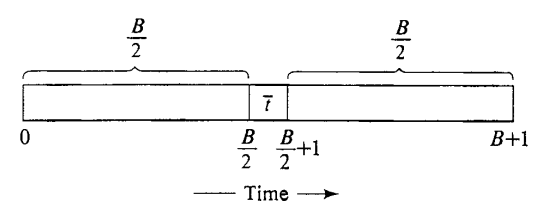
\includegraphics[width=.7\textwidth]{imgs/SWI/SWIdivision.png}
    \end{figure}
    Así el problema de agendación se convierte es un problema de elegir subconjuntos, los que son agendados antes de $\bar{t}$ y los que son agendados después de $\bar{t}$.
\end{frame}

\begin{frame}{Partición = YES =$>$ SWI = YES}
    \begin{itemize}
        \itemj Como la cantidad total de tiempo disponible en los dos bloques es igual al total de la longitud $B$ de las tareas restantes, tenemos que llenar cada bloque de forma exacta.
        \item Esto puede hacerse si y solo si hay un subconjunto $A'\subseteq A$ tal que
        \begin{align*}
            \sum_{a\in A'} s(a) = B/2 = \sum_{a\in A-A'} s(a)
        \end{align*}
        \item Así el subconjunto $A'$ deseado existe para el ejemplar de partición si y solo si existe un horario factible para el ejemplar correspondiente de secuenciación dentro de intervalos.
    \end{itemize}
\end{frame}

\renewcommand{\subsectiontitle}{Ejemplo de transformación}
\subsection{\subsectiontitle}

\begin{frame}{\subsectiontitle}
    Sea $A=\{a_1,a_2,a_3,a_4,a_5,a_6\}$ con $s(a_1)=1,s(a_2)=1,s(a_3)=2,s(a_4)=3,s(a_5)=3,s(a_6)=4$, tenemos que $B=\sum_{1<i<6} s(a_i) = 14$.
    \begin{itemize}
        \itemj Asignamos los valores $r(t_a)=0, d(t_a)=B+1, l(t_a)=s(a)$ para cada $a\in A$:
        
        \vspace{10pt}
        \begin{itemize}
            \item $r(t_{a_1})=0,$ \hspace{5pt} $d(t_{a_1})=B+1=15,$ \hspace{5pt} $l(t_{a_1})=s(a_1)=1$
            \item $r(t_{a_2})=0,$ \hspace{5pt} $d(t_{a_2})=B+1=15,$ \hspace{5pt} $l(t_{a_2})=s(a_2)=1$
            \item $r(t_{a_3})=0,$ \hspace{5pt} $d(t_{a_3})=B+1=15,$ \hspace{5pt} $l(t_{a_3})=s(a_3)=2$
            \item $r(t_{a_4})=0,$ \hspace{5pt} $d(t_{a_4})=B+1=15,$ \hspace{5pt} $l(t_{a_4})=s(a_4)=3$
            \item $r(t_{a_5})=0,$ \hspace{5pt} $d(t_{a_5})=B+1=15,$ \hspace{5pt} $l(t_{a_5})=s(a_5)=3$
            \item $r(t_{a_6})=0,$ \hspace{5pt} $d(t_{a_6})=B+1=15,$ \hspace{5pt} $l(t_{a_6})=s(a_6)=4$
        \end{itemize}

        \item Agregamos la tarea $\bar{t}$  con $r(\bar{t})= \lceil B/2\rceil = \lceil 14/2\rceil = 7$, $d(\bar{t})=\lceil (B+1)/2\rceil=\lceil (14+1)/2\rceil=\lceil 15/2\rceil=\lceil 7.5\rceil = 8$ y $l(\bar{t})=1$.
    \end{itemize}
\end{frame}
\begin{frame}{\subsectiontitle}
    \begin{figure}
    \centering
        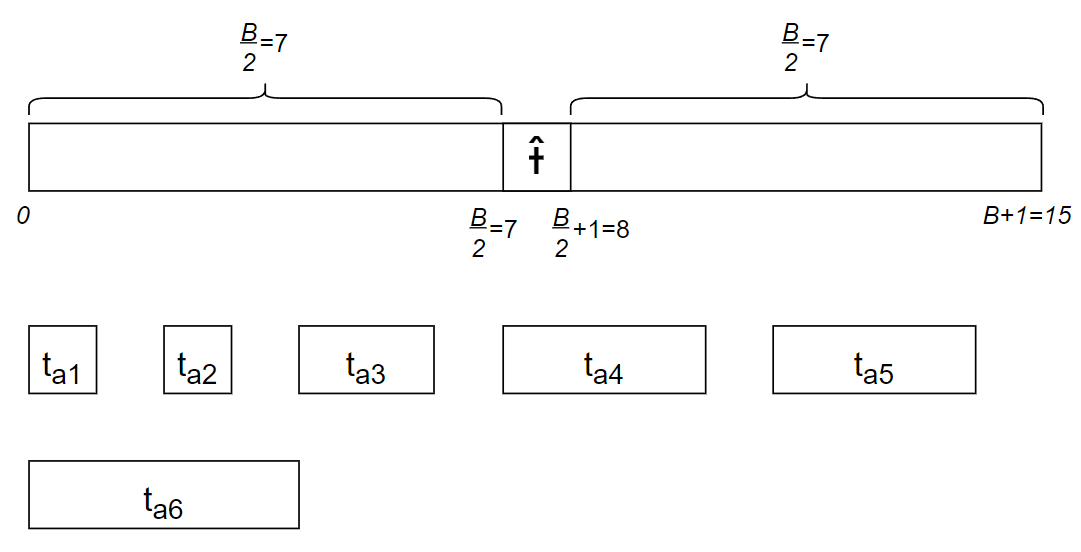
\includegraphics[width=1\textwidth]{imgs/SWI/EjemploSWI_1.png}
    \end{figure}
\end{frame}

\begin{frame}{\subsectiontitle}
    Elegimos el subconjunto $A'=\{a_2,a_3,a_6\}$ y tenemos que $A-A'=\{a_1,a_4,a_5\}$
    \begin{figure}
    \centering
        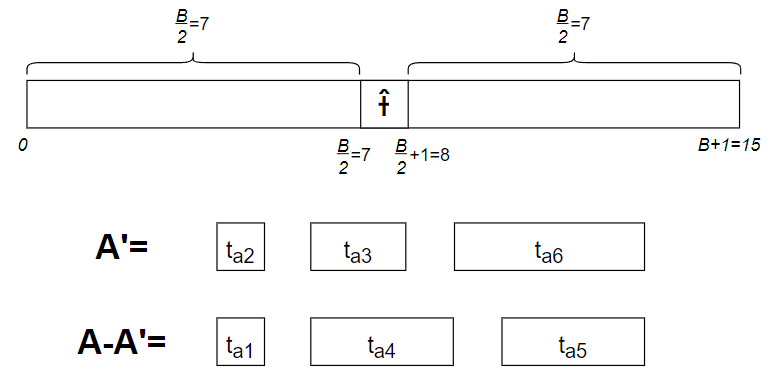
\includegraphics[width=.8\textwidth]{imgs/SWI/EjemploSWI_1_5.png}
    \end{figure}
\end{frame}

\begin{frame}{\subsectiontitle}
    \begin{figure}
    \centering
        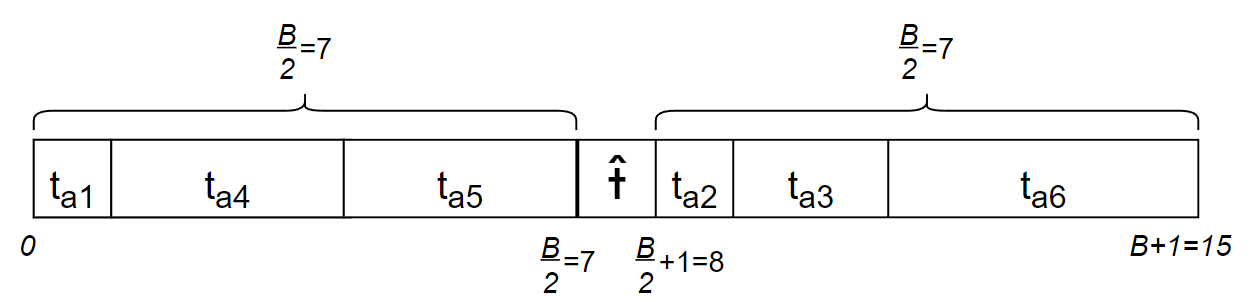
\includegraphics[width=1\textwidth]{imgs/SWI/EjemploSWI_2.png}
    \end{figure}
\end{frame}

\begin{frame}{Aplicaciones en la vida real}
    \begin{itemize}
        \itemj Agendar las tareas que debe realizar una maquina.
        \item Crear horarios bonitos para la escuela.
    \end{itemize}
\end{frame}

%%%%%%%%%%%%%%% FIN PARTE RAG %%%%%%%%%%%%%%%%%%%%%%%

\renewcommand{\sectiontitle}{Multiprocessor Scheduling}
\section{\sectiontitle}
\customToC{currentsection,hideothersubsections}{}
\renewcommand{\subsectiontitle}{Forma canónica o estándar}
\subsection{\subsectiontitle}
\begin{frame}{\subsectiontitle}
\begin{itemize}
    \item \textbf{Ejemplar genérico:} Dado un conjunto de trabajos
        \(\mathcal{J} = \{J_{1}, \dotsc, J_{n}\}\), una gráfica acíclica dirigida 
        \(P = \left(J, A\right)\) \textit{\(A\) es un orden parcial de precedencia}, un entero \(m\) \textit{(el número de procesadores)}
        y un entero \(T\) \textit{(el lapso para cumplir los trabajos de \(\mathcal{J}\))}.
    \item \textbf{Pregunta de decisión:} ¿Existe una función \(S\) de \(\mathcal{J}\) a \(\{1, 2, \dotsc, T\}\), tal que \(S\) cumple con lo siguiente:
    \begin{itemize}
        \item Para todo \(j \leq T \) entonces \(|\{J_{i} \ | \ S\left(J_{i}\right) = j\}| \leq m\)
        \item Sí \(\left(J_{i}, J_{j}\right) \in A\) entonces \(S\left(J_{i}\right) < S\left(J_{j}\right)\)?
    \end{itemize}
\end{itemize}
\end{frame}
\renewcommand{\subsectiontitle}{Entendiendo el enunciado}
\subsection{\subsectiontitle}
\begin{frame}{\subsectiontitle}
\begin{itemize}
    \item Todos los trabajos tardan una unidad de tiempo en ejecutarse.
    \item Los trabajos son la tareas que debe realizar el procesador, como lo puede ser la ejecución de un programa.
    \item El \textbf{orden parcial} quiere decir que hay trabajos los cuales se pueden ejecutar sí y solamente sí los trabajos que los \textbf{preceden} ya han sido ejecutados.
\end{itemize}
\end{frame}
\begin{frame}{\subsectiontitle}
    \begin{itemize}
        \item La restricción de \textit{``Para todo \(j \leq T \) entonces \(|\{J_{i} \ | \ S\left(J_{i}\right) = j\}| \leq m\)``}, nos quiere decir que el número de tareas ejecutados en el tiempo \(j\) son a lo más \(m\), ya que solamente tenemos \(m\) procesadores para realizar las tareas.
        \item La restricción de \textit{``Sí \(\left(J_{i}, J_{j}\right) \in A\) entonces \(S\left(J_{i}\right) < S\left(J_{j}\right)\)``} indica la precedencia de las tareas es decir tenemos que ejecutar primero el trabajo \(J_{i}\) que el trabajo \(J_{j}\) ya que \(J_{i}\) tiene mayor precedencia o su equivalente: \(J_{j}\) no se puede ejecutar hasta que ya se haya ejecutado \(J_{i}\). 
    \end{itemize}
\end{frame}
\renewcommand{\subsectiontitle}{Algoritmo no determinista}
\subsection{\subsectiontitle}
\begin{frame}{\subsectiontitle}
    \begin{itemize}
        \item Fase adivinadora:
        \begin{itemize}
            \item Para la creación de la función \(S\) (recordemos que  $S \ : \ \mathcal{J} \longrightarrow \{ 1, \dotsc, T\}$), damos la siguiente regla de correspondencia:
            \begin{itemize}
                \item Por cada $J \in \mathcal{J}$, tiramos un dado equilibrado de $T$ caras, y el resultado que nos salga sera el lapso para cumplir el trabajo.
            \end{itemize}
            
        \end{itemize} 
        \item Fase verificadora:
        \begin{itemize}
            \item Checamos que cada restricción del problema se cumplan, en caso de que no se cumpla alguna entonces no es una solución. En otro caso sí es una solución para el ejemplar genérico.
        \end{itemize}
    \end{itemize}
\end{frame}
\renewcommand{\subsectiontitle}{Complejidad del algoritmo no determinista}
\subsection{\subsectiontitle}
\begin{frame}{\subsectiontitle}
    \begin{itemize}
        \item Fase adivinadora:
        \begin{itemize}
            \item Tiramos $|\mathcal{J}|$ veces el dado equilibrados de $T$ caras, así la complejidad en tiempo de éste paso está dado por $O\left(|\mathcal{J}|\right)$
            \item Asignarle a cada $J \in \mathcal{J}$ el lapso para cumplir el trabajo tiene complejidad en tiempo de $O\left(|\mathcal{J}|\right)$.
        \end{itemize}
        \item Fase verificadora:
        \begin{itemize}
            \item Definimos al conjunto $C_{j}$ como
            \[
                \{ J_{i} \ | \ S(J_{i}) = j \}
            \]
            es decir, $C_{j}$ es el conjunto de trabajos que están en 
            $\mathcal{J}$ tal que esos trabajos fueron ejecutados en el tiempo $j$.
            \item Comprobar que para un tiempo $j$ tal que $j \leq T$ se cumpla que $|C_{j}| \leq m$ nos toma tiempo $O\left(|C_{j}|\right)$.
            \item Así para todo tiempo $j$ tal que $j \leq T$ se cumpla que $|C_{j}| \leq m$ nos toma tiempo $O\left(T \cdot \sum_{j = 1}^{T} |C_{j}|\right)$.
            \item Comprobar que para todo $(J_{i}, J_{j}) \in A$ se cumpla que
            $S\left(J_{i}\right) < S\left(J_{j}\right)$ tiene complejidad en tiempo de $O\left(|A|\right)$.
        \end{itemize}
    \end{itemize}
\end{frame}
\renewcommand{\subsectiontitle}{Clique}
\subsection{\subsectiontitle}
\begin{frame}{\subsectiontitle}
Definición:
\newline 
Un \textbf{clique} es un subconjunto \(V'\) de vértices de la gráfica \(G = \left(V, E\right)\) tal que sí \( u, v \in V' \) entonces 
\(\left(u, v\right) \in E\)
\end{frame}
\renewcommand{\subsectiontitle}{Ejemplo}
\subsection{\subsectiontitle}
\begin{frame}{\subsectiontitle}
\begin{figure}
    \centering
    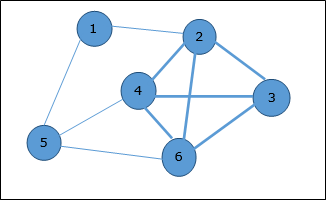
\includegraphics{imgs/MS/Clique/max_cliques.jpg}
    \caption{Gráfica \( G \)}
\end{figure}
\end{frame}
\begin{frame}{\subsectiontitle}
    El conjunto de vértices de \(G\) definido como \( \{2, 4, 6, 3 \} \) es un \textbf{clique} en \(G\) mientras que el conjunto de vértices de \( G \) definido como \( \{ 1, 2, 4 \} \) ya que \( \{ 1, 4 \} \notin E\)
\end{frame}
\renewcommand{\subsectiontitle}{Problema del Clique}
\subsection{\subsectiontitle}
\begin{frame}{\subsectiontitle}
Dada una gráfica \(G\) y un entero \(K\), ¿\(G\) contiene un clique de tamaño al menos \(K\)?
\newline 
El problema del \textbf{clique} es \textbf{NP-}Completo
\end{frame}
\renewcommand{\subsectiontitle}{Teorema}
\subsection{\subsectiontitle}
\begin{frame}{\subsectiontitle}
El problema \textbf{Multiprocessor Scheduling} es \textbf{NP-}Completo.
\end{frame}
\renewcommand{\subsectiontitle}{Demostración}
\subsection{\subsectiontitle}
\begin{frame}{\subsectiontitle}
Transformaremos \textbf{Clique} a \textbf{Multiprocessor Scheduling}.
\newline 
Sea \(G = \left(V, E\right)\) una gráfica tal que:
\begin{itemize}
    \item \(V\) es el conjunto de vértices de la gráfica.
    \item \(E\) es el conjunto de aristras de la gráfica.
\end{itemize}
y sea \(k \in \mathbb{Z}^{+}\) tal que $k \leq |V|$, lo anterior es un ejemplar genérico de \textbf{Clique}.
\newline
Construiremos un conjunto de trabajos \(\mathcal{J}\), una gráfica acíclica \(P = \left(\mathcal{J}, A\right)\) con orden parcial de precedencia
\(A\) y enteros \(m\) y \(T\) de tal manera que existe la función \(S\) de \(\mathcal{J}\) a \(T\) sí y sólo sí \(G\) tiene un \textbf{clique}.
\end{frame}
\begin{frame}{\subsectiontitle}
Supondremos que \(G\) no tiene vértices aislados, ésto no hace que perdamos generalidad ya que los vértices aislados \textit{(los que no tienen aristas incidiendo en ellos)}
podemos eliminarnos de la gráfica y éstos no afectan el tamaño del \textbf{clique} ya que por definición ninguno de éstos vértices aislados forma parte de él.
\newline 
Definimos al conjunto de trabajos \(\mathcal{J}\) de la siguiente manera:
\begin{align*}
    \mathcal{J} &= V \cup E \cup B \cup C \cup D.
\end{align*}
donde \(B, C\) y \(D\) no son \(\varnothing\) y además son disjuntos entre sí. Definimos a los anteriores conjuntos como sigue:
\begin{align*}
    B &= \{b_{1}, \dotsc, b_{|B|}\} \\
    C &= \{c_{1}, \dotsc, c_{|C|}\} \\
    D &= \{d_{1}, \dotsc, d_{|D|}\} \\
\end{align*}
\end{frame}
\begin{frame}{\subsectiontitle}
\(|B|\), \(|C|\) y \(|D|\) satisfacen las siguientes igualdades:
\begin{align*}
    m &= k + |B| = \binom{k}{2} + |V| - k + |C| = |E| - \binom{k}{2} + |D| \\
    min\left(|B|, |C|, |D|\right) &= 1 \\
\end{align*}
A \(T\) se le asigna el valor de \(3\).
\newline 
Para construir la gráfica \(P = \left(\mathcal{J}, A\right) \), iniciamos añadiendo a \(A\) todas las duplas posibles
de la forma \(b_{i}, c_{j}\) y \(c_{j}, d_{k}\). Después agregamos las duplas \(\left(v, e\right)\) para todo 
\(v \in V\) y \(e \in E\) tal que \(e\) incide en \(v\). Ahora tenemos un ejemplar genérico de \textbf{Multiprocessor Scheduling}.
\newline 
\end{frame}
\begin{frame}{\subsectiontitle}
El ejemplar se construyó en tiempo polinomial ya que:
\begin{itemize}
    \item Construir el conjunto \(\mathcal{J}\) está dado por \(O\left(|V| + |E| + |B| + |C| + |D|\right)\).
    \item Construir los números \(m\) y \(T\) se hace en tiempo constante \(O\left(1\right)\) ya que siempre se efectúan el mismo número 
          de operaciones sin importar la cardinalidad de \(B, C, D, E\) y \(V\) en el caso de \(m\).
    \item Construir el conjunto \(A\) está dado por \(O\left(|B| \cdot |C| \cdot |D| + |V| \cdot |E|\right)\).
\end{itemize}
\end{frame}
\begin{frame}{\subsectiontitle}
    \textbf{Afirmación:}
    \newline 
    \textit{Existe la función \(S\) para \(\mathcal{J}\) bajo el orden parcial de precedencia \(A\), con \(m\) y \(T\)
    sí y solamente sí \(G\) tiene un \textbf{clique} de tamaño \(k\)}.
\end{frame}
\begin{frame}{\subsectiontitle}
\textbf{Ida}
\begin{itemize}
    \item Supongamos que existe la función \(S\) del conjunto \(\mathcal{J}\) al conjunto \(\{1, \dotsc, T\}\) tal que cumple:
    \begin{itemize}
        \item Para todo \(j \leq T \) entonces \(|\{J_{i} \ | \ S\left(J_{i}\right) = j\}| \leq m\)
        \item Sí \(\left(J_{i}, J_{j}\right) \in A\) entonces \(S\left(J_{i}\right) < S\left(J_{j}\right)\)
    \end{itemize}
    \item Como \(T = 3\) y por construcción de \(A\) tenemos que todos los trabajos que están en \(B\) deben de ser ejecutados 
    antes que aquellos trabajos están en \(C\) y éstos a su vez se ejecutan primero que los trabajos que están en \(D\).
\end{itemize}
\end{frame}
\begin{frame}{\subsectiontitle}
Necesariamente tenemos que:
\begin{align*}
    S\left(b\right) &= 1 \ \forall b \in B \\
    S\left(c\right) &= 2 \ \forall c \in C \\
    S\left(d\right) &= 3 \ \forall d \in D
\end{align*}
Notemos que:
\[
    |\mathcal{J}| = T \cdot m
\]
Ya que:
\[
    |\mathcal{J}|  = |V| + |E| + |B| + |C| + |D|
\]
porque $V, E, B, C$ y $D$ son todos disjuntos entre sí.
\end{frame}
\begin{frame}{\subsectiontitle}
Por las restricciones que pusimos al contruir a \(m\) tenemos lo siguiente:
\begin{align*}
    |B| &= m - k \\
    |V| + |C| &= m + k - \binom{k}{2} \\
    |D| + |E| &= m +\binom{k}{2}
\end{align*}
\end{frame}
\begin{frame}{\subsectiontitle}
    Así 
    \begin{align*}
        |\mathcal{J}| &= m - k + m + k - \binom{k}{2} + m +\binom{k}{2} \\ 
                      &= m + m + m - k + k  - \binom{k}{2} + \binom{k}{2} \\
                      &= m + m + m = 3 \cdot m \\
    \end{align*}
    como \(T = 3\) entonces 
    \[
        |\mathcal{J}| = T \cdot m
    \]
\end{frame}
\begin{frame}{\subsectiontitle}
    \begin{itemize}
        \item Consecuentemente los \(m\) procesadores siempre están ejecutando algún trabajo durante los \(3\) períodos de ejecución.
        \item Notemos que el último período además de los trabajos que están en el conjunto \(D\) por la restricción de que \(m = |E| - \binom{k}{2} + |D|\)
        tenemos que se ejecutan \(|E| - \binom{k}{2}\) trabajos que corresponden a las aristas de \(G\).
    \end{itemize}
\end{frame}
\begin{frame}{\subsectiontitle}
    \begin{itemize}
        \item Esto es así ya que sí el trabajo 
            correspondiente a un vértice se ejecuta en el último período de ejecución, por construcción el trabajo de las aristas que inciden en ese vértice no se podrían
            ejecutar hasta después del tercer período, es por eso que supusimos que en \(G\) no hay vértices aislados, ya que sí los hubiera, entonces \(S\)
            no existiría con \(T = 3\) como hemos supuesto.
        \item Los \(\binom{k}{2}\) trabajos              restantes corresponden a trabajos          de las aristas que se tienen que           ejecutar en el segundo período.
        \item Los trabajos correspondiente a los         vértices se ejecutan en el primer y        segundo período.
    \end{itemize}
\end{frame}
\begin{frame}{\subsectiontitle}
\begin{itemize}
    \item Como en el primer período se ejecutan todos los trabajos correspondientes a \(B\), también se deben de ejecutar \(k\) trabajos que corresponden \(V\), ésto se debe a la restricción $m = k + |B|$. En el segundo período se ejecutan \(|V| - k\) trabajos que corresponden a los vértices de $G$.
    \item Por lo tanto hemos obtenido lo siguiente:
    \begin{itemize}
        \item En el primer período se ejecutan $k$
        trabajos correspondientes a los vértices.
        \item En el segundo período se ejecutan $\binom{k}{2}$ trabajos correspondientes a las aristas.
    \end{itemize}
\end{itemize}
\end{frame}
\begin{frame}{\subsectiontitle}
    \begin{itemize}
        \item La única manera en que pueda ocurrir lo anterior es que las aristas \textit{(cuyos trabajos correspondientes son ejecutados en el \textbf{segundo período})} sean de la forma $(u, v)$ con 
        $u$ y $v$ vértices cuyos trabajos correspondientes fueron ejecutados en el \textbf{primer período}.
        \item Así para cualquier par de vértices $v'$ y $u'$ de los $k$ vértices existe una arista $(v', u')$, que por definición es un \textbf{clique}.
        \item Por lo tanto en $G$ existe un 
        \textbf{clique} de tamaño $k$.
    \end{itemize}
\end{frame}
\begin{frame}{\subsectiontitle}
\textbf{Regreso}
\newline
Si \(G\) tiene un \textbf{clique} \(V'\) de tamaño \(k\), entonces diseñamos una función \(S\) de la siguiente manera:
\begin{align*}
    S\left(b\right) &= 1 \ \forall b \in B \\
    S\left(c\right) &= 2 \ \forall c \in C \\
    S\left(d\right) &= 3 \ \forall d \in D \\
    S\left(v\right) &= 1 \ \text{sí y sólo sí} \ v \in V' \\
    S\left(v\right) &= 2 \ \text{sí y sólo sí} \ v \notin V' \\
    S\left(\left[v, u\right]\right) &= 2 \ \text{sí y sólo sí} \ v, u \in V' \\
    S\left(\left[v, u\right]\right) &= 3 \ \text{sí y sólo sí} \ v, u \notin V'
\end{align*}
Así \(S\) por construcción cumple con los siguiente:
\begin{itemize}
    \item Para todo \(j \leq T \) entonces \(|\{J_{i} \ | \ S\left(J_{i}\right) = j\}| \leq m\)
    \item Sí \(\left(J_{i}, J_{j}\right) \in A\) entonces \(S\left(J_{i}\right) < S\left(J_{j}\right)\)
\end{itemize}
\end{frame}
\renewcommand{\subsectiontitle}{Ejemplificación de la transformación}
\subsection{\subsectiontitle}
\begin{frame}{\subsectiontitle}
Consideremos la gráfica \(G = \left(V, E\right)\) definida como sigue:
\begin{align*}
    V &= \{v_{1}, v_{2}, v_{3}, v_{4}\} \\
    E &= \{\{v_{1}, v_{2}\},\{v_{1}, v_{3}\}, \{v_{1}, v_{4}\}, \{v_{2}, v_{3}\}, \{v_{3}, v_{4}\}\}
\end{align*}
\begin{figure}[H]
    \centering
    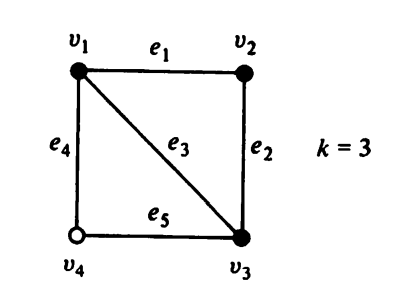
\includegraphics[scale=0.4]{imgs/MS/Ejemplo/ejemp1.png}
    \caption{Gráfica \(G\)}
\end{figure}
\end{frame}
\begin{frame}{\subsectiontitle}
Observemos que:
\begin{align*}
    |V| &= 4 \\
    |E| &= 5
\end{align*}
Redefiniremos a cada arista de \(E\) de la siguiente manera:
\begin{align*}
    e_{1} &= \{v_{1}, v_{2}\} \\
    e_{2} &= \{v_{2}, v_{3}\} \\
    e_{3} &= \{v_{1}, v_{3}\} \\
    e_{4} &= \{v_{1}, v_{4}\} \\
    e_{5} &= \{v_{3}, v_{4}\}
\end{align*}
\end{frame}
\begin{frame}{\subsectiontitle}
Así
\[
    E = \{e_{1}, e_{2}, e_{3}, e_{4}, e_{5}\}  
\]
Un \textbf{clique} de la gráfica \(G\) es el conjunto \(V'\) definado como sigue:
\[
    V' = \{v_{1}, v_{2}, v_{3}\} 
\]
\(|V'| = 3\). Definimos a \(k\) como \(3\).
\end{frame}
\begin{frame}{\subsectiontitle}
Definimos el conjunto \(B\) como sigue:
\[
    B = \{b_{1}, b_{2}\}
\]
Definimos el conjunto \(C\) como sigue:
\[
    C = \{c_{1}\}
\]
Definimos el conjunto \(D\) como sigue:
\[
    D = \{d_{1}, d_{2}, d_{3}\}
\]
Notemos que los conjuntos \(B, C, D\) son disjuntos.
\newline 
De lo anterior obtenemos que:
\begin{align*}
    |B| &= 2 \\
    |C| &= 1 \\
    |D| &= 3 \\
\end{align*}
\newline 
\end{frame}
\begin{frame}{\subsectiontitle}
Definimos a \(m\) como sigue:
\begin{align*}
    m &= k + |B| \\
    m &= \binom{k}{2} + |V| - k + |C| \\
    m &= |E| - \binom{k}{2} + |D|
\end{align*}
Sustituyendo
\begin{align*}
    m &= 3 + 2 = 5 \\
    m &= 3 + 4 - 3 + 1 = 5 \\
    m &= 5 - 3 + 3 = 5
\end{align*} 
Notemos que también las cardinalidades de los conjuntos \(B, C, D\) cumplen con:
\[
    \text{mín}\left(|B|, |C|, |D|\right) = 1
\]
\end{frame}
\begin{frame}{\subsectiontitle}
Calcularemos \(B \times C\)
\begin{align*}
    B \times C &= \{(b_{1}, c_{1}), (b_{2}, c_{2})\}
\end{align*}
Calcularemos \(C \times D\)
\begin{align*}
    C \times D &= \{(c_{1}, d_{1}), (c_{1}, d_{2}), (c_{1}, d_{3})\}
\end{align*}
\end{frame}
\begin{frame}{\subsectiontitle}
Orden parcial de los trabajos que están en los conjuntos \(B, C\) y \(D\)
    \begin{figure}
    \centering
    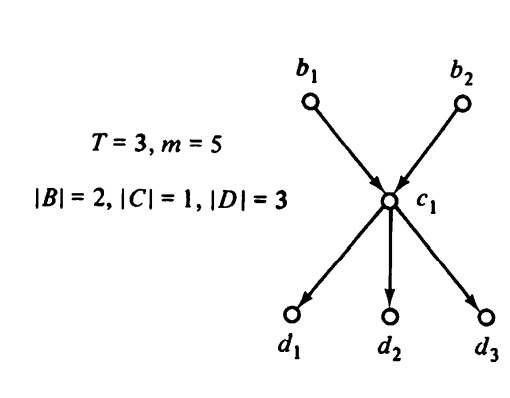
\includegraphics[scale=0.45]{imgs/MS/Ejemplo/ejemp2.png}
    \label{fig:my_label}
\end{figure}
\end{frame}
\begin{frame}{\subsectiontitle}
Sea \(A'\) el conjunto definido como sigue:
\begin{align*}
    A' &= \{(v, e) \ | \ v \in V, e \in E \ \text{tal que \(e\) incide en \(v\)}\} \\
    A' &= \{(v_{1}, e_{1}), (v_{1}, e_{3}), (v_{1}, e_{4}), (v_{2}, e_{1}), (v_{2}, e_{2}), (v_{3}, e_{3}), (v_{3}, e_{5}), (v_{4}, e_{4}), (v_{4}, e_{4}) \}
\end{align*}
Definimos a \(A\) como 
\[
    A = B \times C \cup C \times D \cup A'
\]
\(A\) lo tomaremos como un orden parcial de precedencia.
\newline 
\end{frame}
\begin{frame}{\subsectiontitle}
Orden parcial de los trabajos que están en los conjuntos \(V\) y \(E\)
    \begin{figure}
        \centering
        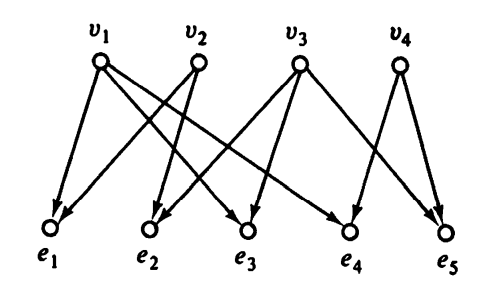
\includegraphics[scale=0.5]{imgs/MS/Ejemplo/ejemp3.png}
    \end{figure}
\end{frame}
\begin{frame}{\subsectiontitle}
    \begin{itemize}
        \item Por lo tanto hemos convertido un ejemplar particular de \textbf{Clique} en un ejemplar particular de \textbf{Multiprocessor Scheduling}.
    \end{itemize}
\end{frame}
\renewcommand{\subsectiontitle}{Técnica para la demostración del problema}
\subsection{\subsectiontitle}
\begin{frame}{\subsectiontitle}
\begin{itemize}
    \item Reemplazo Local
\end{itemize}
\end{frame}
\renewcommand{\subsectiontitle}{Aplicación en la vida real}
\subsection{\subsectiontitle}
\begin{frame}{\subsectiontitle}
\begin{itemize}
    \item Encontrar una manera eficiente por parte del \textbf{Sistema Operativo} de ejecutar tareas en los múltiples procesadores de la computadora.
\end{itemize}
\end{frame}

% Import bibliography from file sample.bib
\begin{frame}[t, allowframebreaks]
\frametitle{Referencias}
\begin{thebibliography}{10}
\bibitem{garey79}
\alert{Garey. M.R and Johnson, D. S}
\newblock  {Computer and intractability. A guide to the Theory of NP-Completness}
\newblock {\em W.H. Freeman and Company. New York (1979), 66-72}.

\bibitem{papadimitriou82}
\alert{Papadimitriou, Ch}
\newblock {Combinatorial Optimization: Algorithms and Complexity}
\newblock {\em Dover Publications, INC. Mineola, New York (1982), 363-366}.
\end{thebibliography}

\end{frame}

\end{document}